\documentclass{prova}

\usepackage{amsmath}

\newcommand{\sen}{\mbox{sen}\,}
\newcommand{\ds}{\displaystyle}

\professor{Prof.\@ Adriano Barbosa}
\disciplina{C\'alculo Diferencial e Integral III}
\avaliacao{P2}
\curso{Engenharia de Alimentos}
\data{12/06/2019}

\begin{document}
	\cabecalho{5}  % o numero 5 indica a qnt de quadros na tabela de nota

	\textbf{Todas as respostas devem ser justificadas.}
    \vspace{1cm}

	\begin{questionario}
        \q{Calcule a integral dupla $\ds\int_0^2\int_{x^2}^{2x} x^2+y^2\ dy\ dx$.}
        \q{Calcule a integral $\ds\iint_R \sen{(x^2+y^2)}\ dA$, onde $R$ \'e a
        regi\~ao do primeiro quadrante entre os c\'{\i}rculos com centro na origem e
        raios 1 e 3. (Dica: use coordenadas polares)}
        \q{Calcule $\ds\iiint_E \sqrt{x^2+y^2}\ dV$, onde $E$ \'e a regi\~ao
        delimitada pelo cil\'{\i}ndro $x^2+y^2=1$ e pelos planos $z=-1$ e $z=2$.}
            \begin{figure}[h]
                \centering
                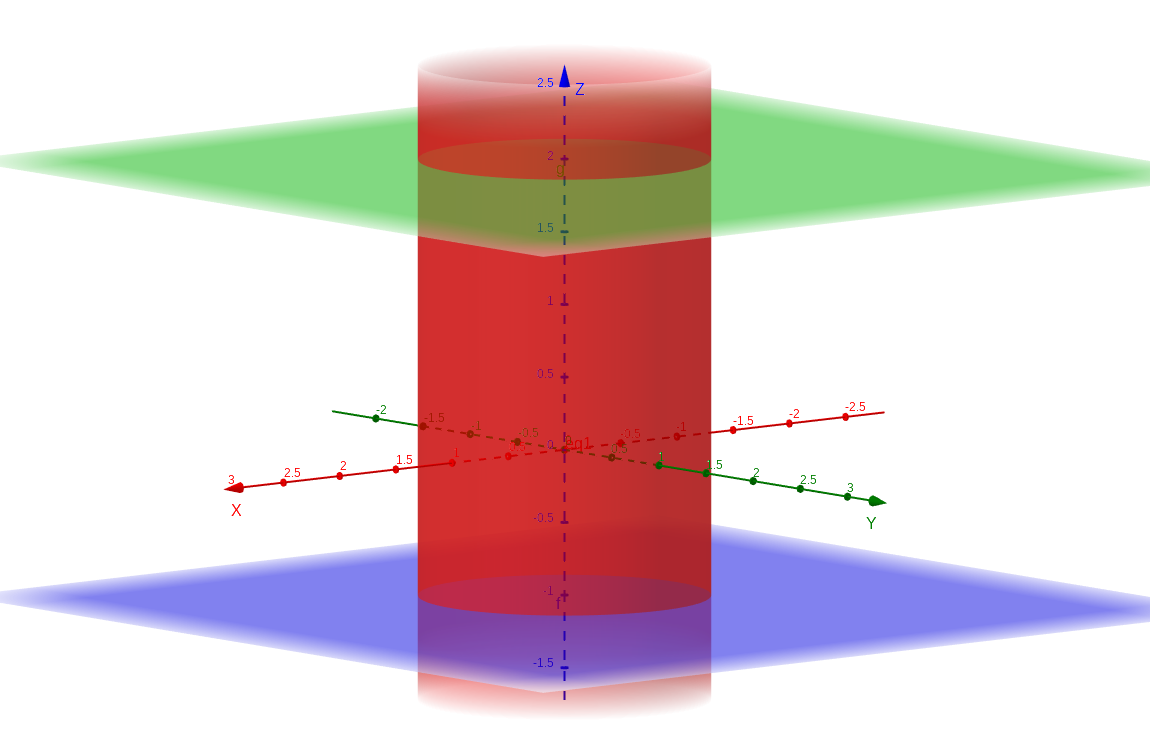
\includegraphics[width=0.5\textwidth]{q3.png}
            \end{figure}
        \q{Calcule o trabalho realizado pelo campo $F(x,y) = (xy^2,x^2y)$
        ao mover uma part\'{\i}cula de $(0,0)$ a $(2,1)$.}
        \q{Calcule a integral de linha $\ds\int_C xy\ dx + x^2y^3\ dy$, onde $C$ \'e
        o tri\^angulo com v\'ertices $(0,0)$, $(1,0)$ e $(1,2)$.}
	\end{questionario}
\end{document}
